\documentclass[twocolumn,twoside,a4paper, 10pt]{article}
\usepackage[utf8]{inputenc}
\usepackage[T1]{fontenc}
\usepackage[spanish]{babel}
\usepackage{balance}
\usepackage{jenuia4}
\usepackage{url}
%\usepackage{graphicx}

% Mis paquetes. No incluídos en la plantilla de Jenui
\usepackage{hyperref}
\usepackage{float} % For float Listings
\usepackage[pdftex]{color}
\usepackage[pdftex]{graphicx}
%\graphicspath{{FIGURES/png/}} 
%%%%%%%%%%%%%%%%%%%%%%%%%%%%%%%%%%%%%%%%%%%%%%%%%%%%%%%%%%%%%%%%%%%%%%%%%%%%%%%%%%%%%%%%%%%%%
\definecolor{marron}       {rgb}{0.496, 0.203, 0.152}
\definecolor{verde-claro}  {rgb}{0.625, 0.734, 0.199}
\definecolor{oscuro}       {rgb}{0.187, 0.141, 0.285}
\definecolor{gris}     	   {rgb}{0.500, 0.500, 0.500}
\definecolor{bgd-listings} {rgb}{0.999, 0.999, 0.900}
\definecolor{gray97}{gray}{.97}
\definecolor{gray75}{gray}{.75}
\definecolor{gray45}{gray}{.45}
%%%%%%%%%%%%%%%%%%%%%%%%%%%%%%%%%%%%%%%%%%%%%%%%%%%%%%%%%%%%%%%%%%%%%%%%%%%%%%%%%%%%%%%%%%%%%
%% Para listados de código
\usepackage{listings} 
\lstset{language=C++,
        basicstyle=\scriptsize\ttfamily,
        commentstyle=\color{blue},           % comentarios en azul
        keywordstyle=\bfseries,
        stringstyle=\color{red}\ttfamily,
        morecomment=[l][\color{magenta}]{\#}
        framexleftmargin=5mm,									% BGD: Margen izquierdo de los marcos (para que quepan num. de línea) 
        frame=trbl,														% BGD: Cuadro  (t/T: top, r/R: right, b/B: bottom, l/L: left): x->thin, X->thick
        framesep=4pt,
}
%\usepackage{listings} 
%\lstloadlanguages{C++}
%\lstset{
%  language=C++,                        % C
%  keywordstyle=\color{red},            % Palabras clave en rojo
%  identifierstyle=\ttfamily,
%  commentstyle=\color{blue},           % comentarios en azul
%  stringstyle=\color{green},           % cadenas en verde
%	%showstringspaces=false
%  language=C,                          	% C
%  %backgroundcolor=\color{bgd-listings},
%	%backgroundcolor=\color{yellow},     	% Códigos sobre fondo amarillo
%	%frame=lines,                        	% Línea arriba y abajo de cada listado de código
%  %framerule=0pt,
%  %basicstyle=\small\ttfamily,
%	basicstyle=\scriptsize,                   	% Listados en tiny
%	captionpos=b,													% Posición de los títulos abajo (bottom)
%  keywordstyle=\bfseries,
%	%keywordstyle=\color{black}\textbf,   	% BGD: Palabras clave en negro y negrita
%	identifierstyle=\color{black}\ttfamily, % BGD: Identificadores en negro	
%	commentstyle=\color{blue}\textit,  	 	% BGD: Comentarios en azul cursiva
%  stringstyle=\ttfamily,
%	%stringstyle=\color{red}\texttt,       % BGD: Cadenas en rojo
%	directivestyle=\color{oscuro}\texttt,	
%  emph={pragma,llc,omp},								% BGD: Resaltar las palabras pragma, llc y omp
%	emphstyle=\textbf,
%	showstringspaces=false,								% BGD: No mostar espacios
%	columns=fixed,
%	basewidth={0.6em, 0.45em},
%	xleftmargin=5mm,
%	keepspaces=true,											% BGD: Mantener espacios
%	framexleftmargin=5mm,									% BGD: Margen izquierdo de los marcos (para que quepan num. de línea) 
%	frame=trbl,														% BGD: Cuadro  (t/T: top, r/R: right, b/B: bottom, l/L: left): x->thin, X->thick
%	framesep=4pt,
%	%frameround=fttt,											% BGD: Cuadro con esquina curvadas
%  %framextopmargin=3pt,
%  %framexbottommargin=3pt,
%  %framexleftmargin=0.4cm,
%  %framesep=0pt,
%	rulesepcolor=\color{black},						% BGD: Color de los cuadros azul
%	numbers=left,													% BGD: Números de línea a la izquierda
%	firstnumber=1,												% BGD: Número línea empieza en 0 (línea vacía, no se muestra)
%	stepnumber=1,													% BGD: Números línea a línea
%	numberstyle=\scriptsize,										% BGD: Números de línea pequeños
%	numbersep=8pt,												% BGD: Números de línea separados 8 pts a la izquierda
%	numberblanklines=false,								% BGD: No pone números de línea en líneas vacías
%	extendedchars=true,									  % BGD: Utiliza caracteres extendidos (tildes, etc.)
%	inputencoding=latin1,									
%  %inputencoding=utf8x,									
%	tabsize=2,														% BGD: Tamaño de tabulador para indentaciones = 2
%	breaklines=true,											% BGD: Cortar líneas si son muy grandes
%	breakautoindent=true,									% BGD: Autoindentar líneas cortadas
%	postbreak=\space											% BGD: Cortar líneas por espacios
%}

%% minimizar fragmentado de listados
%\lstnewenvironment{listing}[1][]
%   {\lstset{#1}\pagebreak[0]}{\pagebreak[0]}
%\lstdefinestyle{consola}
%   {basicstyle=\scriptsize\bf\ttfamily,
%    backgroundcolor=\color{gray75},
%   }
%\lstdefinestyle{C}
%   {language=C,
%   }
%%%%%%%%%%%%%%%%%%%%%%%%%%%%%%%%%%%%%%%%%%%%%%%%%%%%%%%%%%%%%%%%%%%%%%%%%%%%%%%%%%%%%%%%%%%%%
\AtBeginDocument{
  %\renewcommand\thelstlisting{\arabic{chapter}.\arabic{section}}
  \renewcommand{\thelstlisting}{\arabic{lstlisting}}
}
\renewcommand{\lstlistingname}{Listado} % Los títulos de los códigos insertados se denotan con "Listado"
%%%%%%%%%%%%%%%%%%%%%%%%%%%%%%%%%%%%%%%%%%%%%%%%%%%%%%%%%%%%%%%%%%%%%%%%%%%%%%%%%%%%%%%%%%%%%
\newcommand{\jutge}{\textit{Jutge.org}{}}           % BGD: Nuevos comandos para imprimir con estilo
\newcommand{\ChatGPT}{\textit{ChatGPT}{}}           % BGD: Nuevos comandos para imprimir con estilo
%%%%%%%%%%%%%%%%%%%%%%%%%%%%%%%%%%%%%%%%%%%%%%%%%%%%%%%%%%%%%%%%%%%%%%%%%%%%%%%%%%%%%%%%%%%%%
\title{El impacto de asistentes basados en IA en la enseñanza-aprendizaje de la programación}
%\author{\normalsize 
%\begin{tabular}{@{\extracolsep{3mm}}cc}
%{\large Joe Miró Julià }                  & {\large Mercedes Marqués}\\
%Departament de Matemàtiques i Informàtica & Departamento de Ing. y Ccia. de los Comput.\\
%Universitat de les Illes Balears          & Universitat Jaume I\\
%07122 Palma de Mallorca                   & Castellón\\
%\url{joe.miro@uib.es}                     & \url{merche.marques@uji.es}
%\end{tabular}
%}

\author{ \small
\begin{tabular}{@{\extracolsep{3mm}}c}
\large Francisco de Sande \\
Departamento de Ingeniería Informática y de Sistemas \\
Universidad de La Laguna \\
38200 La Laguna. S/C de Tenerife \\
fsande@ull.es
\end{tabular}
}

\date{}

%%%  Referencias
% https://aihub.csic.es/inteligencia-artificial-en-educacion-golem-creativo-o-destructor/

\begin{document}
\maketitle
\thispagestyle{empty}

\begin{abstract}
\noindent Abstract
\end{abstract}

\section*{Abstract}
\noindent Abstract 

\section*{Palabras clave}
\noindent Programación IA ChatGPT GitHub Copilot Enseñanza Informática Evaluación

\section{Introducción}
La programación es una actividad transversal a cualquier rama de la informática y su
importancia es compartida por cualquier especialización en esta titulación.
\textit{Informática Básica} (IB, de ahora en adelante) es la primera asignatura en la que el alumnado toma 
contacto con esta materia y en la que ha de aprender los fundamentos de la misma.
Los conceptos objeto de estudio son comunes, con pequeñas variaciones, a cualquier lenguaje de programación
orientado a objetos, que es el paradigma objeto de estudio en IB.

IB es una asignatura de 6 créditos que se imparte en el primer cuatrimestre 
del primer curso del Grado en Ingeniería Informática en la Escuela Superior de Ingeniería y Tecnología de la
Universidad de La Laguna.
Se trata de la primera asignatura (y única en ese primer  cuatrimestre) de perfil eminentemente informático que
cursa el alumnado del título de Grado.

El número de estudiantes que habitualmente cursa la asignatura está en torno a los 250. 
Los contenidos de la asignatura pueden consultarse en la Guía Docente
%\cite{ULL:2022:GD} 
\footnote{Guía Docente de IB\\ \href{https://www.ull.es/apps/guias/guias/view_guide/34182/}{\scriptsize{\texttt{https://www.ull.es/apps/guias/guias/view\_guide/34182/}}}}.
de la misma.
Al margen de tres temas dedicados a una introducción a las Bases de Datos, Redes y Sistemas Operativos,
el grueso de los contenidos (en torno a 12 de las 15 semanas del cuatrimestre) se dedican a introducir al
alumnado en la materia de Programación, siendo C++ el lenguaje vehicular elegido para estudiar la materia.
Se trata de una asignatura con una importante proporción de contenidos prácticos en la que cada estudiante
recibe 4 horas presenciales de clase a la semana distribuídas del siguiente modo:
\begin{itemize}
  \item 2 horas dedicadas al estudio de contenidos teóricos
  \item 1 hora dedicada a la resolución de Problemas
  \item 1 horas de Prácticas
\end{itemize}
Se describe a continuación el tipo de actividades que se desarrolla en cada una de este tipo de sesiones.

Las sesiones destinadas a contenidos teóricos se imparten con el formato de clase expositiva y se dedican, 
con el uso de transparencias que el alumnado tiene disponibles a través del aula virtual, al estudio de los 
contenidos de la asignatura. 
Junto a las transparencias, el alumnado dispone de una serie de pequeños programas que sirven de ilustración a
los contenidos que se estudian en clase. 
Se recomienda al alumnado estudiar esos programas para afianzar sus conocimientos de cada tema.

En las sesiones de problemas el profesorado utiliza un terminal cuya pantalla se proyecta a toda la clase para
resolver algunos problemas seleccionados, resolviendo al mismo tiempo las dudas que puedan surgir en esa
resolución. 

La Guía docente establece que por cada hora de trabajo presencial, cada estudiante debería dedicar en 
promedio 1,5 horas de trabajo autónomo, de modo que se espera unas 6 horas de trabajo autónomo semanal por 
parte de cada estudiante. 
A pesar de que el peso de los contenidos prácticos de la asignatura suponen solo un 20\% del total de la
calificación de la asignatura, se espera que la mayor parte de ese tiempo se destine al diseño y desarrollo 
de programas de complejidad creciente conforme avanza el desarrollo del curso, y que se evalúan en las
sesiones prácticas.

Cada semana al alumnado se le propone la realización de una práctica, consistente en un cierto número (cinco
es un número habitual) de programas en C++ relacionados con algún tema estudiado.
Esos programas tienen el propósito de servir de ``entrenamiento'' para que el alumnado afiance conocimientos a
lo largo de la semana de la que disponen para realizar esos ejercicios.
La sesión semanal de prácticas se destina a la evaluación de esos conocimientos a través de la realización de
ejercicios de programación de complejidad similar a los que han sido propuestos con antelación.
En las últimas prácticas de la asignatura los ejercicios de evaluación suelen ser simples modificaciones de 
los que se han propuesto para realizar con antelación.

% 10 minutos para cuestionarios

\section{Motivación}
Más allá del ineludible aprendizaje de los conceptos básicos de la materia, 
es un hecho bien conocido que la práctica es fundamental para aprender a programar ordenadores. 
Habitualmente el profesorado asigna problemas de programación al alumnado para ayudarles a adquirir esta 
destreza, y el incremento de las habilidades de una programadora pasa ineludiblemente por muchas horas de dedicación 
a la realización de programas de complejidad creciente.
Forzando un poco las similitudes podríamos decir que la programación se asemeja a las habilidades para
conducir un automóvil: cualquier persona con permiso para conducir puede decir que conduce correctamente, pero
acreditar que se es una buena conductora requiere muchas horas de práctica y exposición a situaciones
infrecuentes.
Del mismo modo cualquier informático dirá que sabe programar pero sus habilidades en esta materia dependerán
muy directamente de las horas de práctica que haya dedicado a la misma.
Siguiendo esta idea, recomendamos encarecidamente al alumnado de IB que realice cuantos ejercicios prácticos
sean capaces para, de forma progresiva, ir incrementando sus capacidades como programadoras.

Las prácticas de la asignatura se convierten pues en una oportunidad para que el alumnado mejore destrezas y
habilidades que le capaciten para abordar los contenidos de asignaturas de cursos posteriores de la
titulación.

La masificación de los grupos de laboratorio de prácticas, con grupos de hasta 20 estudiantes por sesión son
la mayor dificultad para la evaluación de esos trabajos prácticos.
Esta dificultad es compartida por muchas otras asignaturas de la titulación que tienen una significativa
componente práctica en sus contenidos, de modo que casi todas las cuestiones que en este trabajo queremos
plantear son comunes a muchas asignaturas e incluso a otras titulaciones.

Una vez realizadas tres prácticas iniciales en las que el alumnado se familiariza con el Sistema Operativo
Linux, con el entorno de máquina virtual en el que desarrollará sus programas y con el editor \texttt{vim}, 
que es el que se utiliza inicialmente, todas las prácticas restantes abordan contenidos de programación que
cubren los siguientes tópicos:
\begin{itemize}
  \item Primeros programas y conceptos básicos
  \item Expresiones y tipos de datos
  \item Alternativas
  \item Iteraciones
  \item Funciones
  \item Cadenas de texto (\texttt{std:string})
  \item \texttt{std::array} y \texttt{std::vector}
  \item Ficheros
  \item Introducción a la Programación Orientada a Objetos
\end{itemize}

Desde hace ya varios cursos en IB se viene usando la plataforma \jutge{} (juez) 
\cite{Petit:Jutge:2018} para la evaluación de las prácticas.
Se trata de una plataforma que ha sido desarrollada en la Universidad Politécnica de Catalunya,
diseñada tanto para profesorado como para alumnado.
La plataforma aloja una gran cantidad de problemas (aproximadamente unos 2100) que cubren diversidad de
tópicos incluyendo entre ellos los fundamentos de la programación.
Los problemas están perfectamente descritos y contienen un conjunto de tests que el código de usuario ha de
verificar.
Como una de sus características, \jutge{} hace hincapié en el trabajo del alumno, por lo que 
resulta especialmente útil para reforzar el enfoque de aprender haciendo, en nuestro caso, programando.

El modo de funcionamiento de \jutge{} requiere que cuando un estudiante resuelve un problema suba el código
fuente de su solución a la plataforma
\footnote{\textit{Jutge.org} Home Page \href{https://jutge.org/}{\scriptsize{\texttt{https://jutge.org/}}}}
donde se comprueba que sea correcta pasando los correspondientes tests, de los cuales algunos son públicos
y otros privados.
A una solución se le asigna el veredicto AC (\textit{Accepted}) cuando pasa todos los tests existentes para el problema.
En su cuenta de \jutge{} cada estudiante dispone de un cuadro de mandos en el que se recopila el número de
envíos que ha realizado, el de problemas aceptados y rechazados así como diversos gráficos que muestran la
evolución en su trabajo con los problemas de la plataforma.

Este modo de trabajo se aprovecha en las prácticas de IB: en cada sesión de evaluación se le pide al alumnado
que resuevla un pequeño número de problemas (programas) de \jutge{}.
La evaluación de la sesión depende no solo del número de problemas resuelto (no suelen ser más de dos o tres)
sino de la calidad del código desarrollado.
\jutge{} comprueba exclusivamente que el código evaluado funcione correctamente, mientras que en IB se
enfatizan otros aspectos del código que nos parecen tanto o más relevantes que el propio funcionamiento del
mismo, que obviamente es un requisito ineludible.
Muchos de los requisitos que se exigen a los programas de prácticas de IB se definen en la Guía de estilo de 
referencia que se sigue en la asignatura 
%\cite{Google::GSG}
\footnote{Google C++ Style Guide\\ \href{https://google.github.io/styleguide/cppguide.html}{\scriptsize{\texttt{https://google.github.io/styleguide/cppguide.html}}}}.

Relacionamos a continuación algunos de los requisitos exigidos, que obviamente se introducen al alumnado de
forma progresiva:
\begin{itemize}
\item Correcto sangrado del código
\item Adecuado uso de espacios y signos de puntuación en el código
\item Adhesión a las reglas de nombrado de identificadores de variables, funciones, clases, etc.
\item Que todos los identificadores utilizados (salvo excepciones puntuales) sean significativos, evitando el
  uso de ``identificadores de un único carácter''.
\item Que todos los ficheros, funciones y métodos del código incluyan un breve prólogo con comentarios en
  formato Doxygen exponiendo la información más relevante sobre el elemento (función, clase, fichero, ...) en
    cuestión.
\item Que la compilación de todos los programas se automatice mediante el uso de herramientas como
  \texttt{make} o \texttt{cmake}.
\item Que los parámetros de tipos estructurados que se pasen a una función/método estén sean referencias
  constantes.
\item Que los métodos definidos en las clases de los programas sean \textit{const friendly}.
\end{itemize}

Un problema recurrente en todas las asignaturas que requieren la evaluación de prácticas de programación es la
infracción por parte de algunos estudiantes de las reglas de código de conducta que establecen que los
trabajos presentados a evaluación han de ser programas originales realizados por sus autores.
Ante la dificultad de acreditar fehacientemente esta restricción en una sesión de evaluación con un elevado
número de estudiantes en el aula de prácticas y con un tiempo tan limitado se ha optado por valorar
casi exclusivamente el trabajo que el estudiante realiza \textit{in situ} en la sesión de evaluación, y no los
ejercicios que durante la semana ha realizado en calidad de preparación para esa evaluación.


En junio de 2021, GitHub lanzó \textit{Copilot} 
%\cite{Friedman:2021:IGC}
%\cite{Dakhel:2022:GCA},
\cite{Nguyen:2022:AnEE},
un ``programador de pares de IA'' que genera 
código en diversos lenguajes a partir de cierto contexto como comentarios, nombres de funciones y código adyacente. 
\textit{Copilot} se basa en un modelo que se entrena con código abierto \cite{Chen:2021:ELL}.

En febrero de 2022 \textit{DeepMind} publicó \textit{Alphacode}, un sistema basado en Inteligencia Artificial
(IA) que puede competir con un humano en la resolución de problemas sencillos de programación.
Según resultados publicados en \textit{Sience} \cite{Li:2022:CCG}, \textit{Alphacode} gana en un 50\%
de ocasiones a humanos en competiciones de resolución de problemas de programación.

El pasado 30 de noviembre, \textit{OpenAI} lanzó \ChatGPT{}
\cite{Zhang:2020:chatgpt, Castelvecchi:2022:ACaA}, un \textit{chatbot} interactivo de propósito general.
Tanto \ChatGPT{} como \textit{AlphaCode} son ``grandes modelos lingüísticos'', es decir, sistemas basados en 
redes neuronales que aprenden a realizar una tarea a partir de cantidades ingentes de texto generado por humanos. 
De hecho, ambos sistemas utilizan prácticamente la misma arquitectura, siendo la principal diferencia entre
ellos el conjunto de datos con que son entrenados, lo cual los dirige a diferente tipo de tareas.
\ChatGPT{} está basado en el modelo GPT-3.5 que se ajusta con técnicas de aprendizaje supervisado y de
refuerzo y su lanzamiento ha causado enorme interés tanto en la comunidad informática como en medios de
comunicación generalistas \cite{Perez:2022:FBM} y atrayendo la atención de más de un millón de usuarios tan solo 
cinco días depués de su lanzamiento.




con patrones de codificación inseguros, lo que da lugar a la posibilidad de sintetizar código que contenga 
estos patrones indeseables".


\section{Experiencias con \ChatGPT{}}
Todos los enunciados de problemas de \jutge{} están públicamente disponibles en la
plataforma 
%\cite{URL::prob} 
\footnote{Jutge Problems \href{https://jutge.org/problems/}{\scriptsize{\texttt{https://jutge.org/problems/}}}}
y cada uno de ellos cuenta con una descripción clara y precisa así como un
conjunto de tests públicos.

Consideremos a modo de ejemplo el problema \textit{Primality} (P48713).
Se trata de determinar si cada uno de los números naturales de una secuencia es o no primo.
Si el enunciado del problema, junto con los tests se le pasan a \ChatGPT{} en inglés, tal como figuran en
\jutge{}, la solución que obtiene es la más habitual para un programador inexperto, la de fuerza bruta 
consistente en probar todos los divisores en el rango $[2, N-1]$.
Esta solución no recibe el veredicto ``\textit{Accepted}'' en \jutge{} sino que la plataforme indica
como veredicto \textit{Execution Error (time limit exceeded)}.
Ello se debe a que espera un algoritmo más eficiente para este cómputo.

Esta solución es la que cabría esperar de un estudiante de primer curso de informática.
Con frecuencia observamos estudiantes que ofrecen un algoritmo óptimo y ello es una pista para detectar que,
posiblemente han hallado la solución en algún foro. 
Al preguntar al estudiante la razón por la que no recorre todo el rango de búsqueda cabría esperar una
respuesta en la que el estudiante indique que ha investigado el problema y aprendido sobre el mismo, pero es
frecuente una respuesta del tipo ``\textit{lo he probado y he observado que funcionaba}'', que obviamente no se
considera adecuada para la evaluación de un ejercicio práctico.

En el propio enunciado del problema se indica una pista para un algoritmo de menor complejidad.
Si a \ChatGPT{} (en este caso en inglés) se le indica
\textit{Could you optimize the is\_prime() function for a better performance?}
el bot modifica la función, entregando en este caso una versión que sí es aceptada en \textit{Jutge.org}.
A pesar de haberlo indicado en el enunciado del problema, la función entregada no cumple con el convenio que
establece la Guía de Estilo de Google, pero si se le indica esa circunstancia, el bot corrige el identificador
de la función. 
El código completo de la función es el que se muestra en el Listado \ref{code:prime}.
%%%%%%%%%%%%%%%%% Code %%%%%%%%%%%%%%%%%%%%%%%%%%%%%%%%%%%%%
\begin{figure*}[t]
%\begin{lstlisting}[firstnumber=1,caption={Test de primalidad suministrado por \ChatGPT{}},label=code:mandel_seq,float=[htb]]
%\begin{lstlisting}[firstnumber=1,caption={Test de primalidad suministrado por \ChatGPT{}},label=code:prime,float,floatplacement=tbph]
\begin{lstlisting}[caption={Test de primalidad suministrado por \ChatGPT{}. Complejidad $O(\sqrt(n))$},label=code:prime]
/**
 * @brief Function that determines if a given number is prime or not.
 *
 * @param number The number to check for primality.
 * @return true if the number is prime, false otherwise.
 */
bool IsPrime(int number) {
  if (number <= 1) return false;  // 1 and 0 are not considered prime.
  if (number <= 3) return true;  // 2 and 3 are prime.
  if (number % 2 == 0 || number % 3 == 0) return false;  // Check for divisibility by 2 and 3.
  for (int i = 5; i * i <= number; i += 6) {  // Check for divisibility by numbers of the form 6k +/- 1.
    if (number % i == 0 || number % (i + 2) == 0) return false;
  }
  return true;
}
\end{lstlisting}
\end{figure*}
%%%%%%%%%%%%%%%%%%%%%%%%%%%%%%%%%%%%%%%%%%%%%%%%%%%%%%%%%%%

En el caso de \textit{Primality}, en una sesión diferente con \ChatGPT{} se le ha entregado el enunciado en español y
en ese caso, el bot entrega directamente la solución con la optimización del código, pero el código no cumple
con el estándar de Estilo en cuanto a la colocación de las llaves de apertura y cierre de bloques en C++.

\section{Bibliografía}
En el texto se utiliza el número de la referencia, también entre 
corchetes. Hay tres cuestiones a tener en cuenta: (a) El número de 
referencia no puede empezar una línea, hay que poner un ``blanco 
duro'' entre el número de referencia y el texto que lo precede; (b) 
Si hay varias referencias juntas debe usarse un único par de 
corchetes: debe ser ``[2, 7, 14]'' y no ``[2][7][14]''; (c) Si hay 
varias referencias, deben ir en orden numérico ascendente: debe ser  
``[2, 7, 14]'' y no ``[14, 2, 7]''.

El formato de la bibliografía casi merece un artículo propio. 
Recomendamos que las referencias bibliográficas se incluyan en un fichero 
independiente así como el uso del estilo \textit{jenui}. Éste es una adaptación al castellano 
del clásico estilo \textit{plain}.
Si se usa un programa bibliográfico como BibTeX, o EndNote no es necesario 
preocuparse de mucho. En cambio, si se crea la bibliografía a mano 
recomendamos que se mire este artículo o un libro adecuado como 
referencia y que se sigan las siguientes normas:
%
\begin{itemize}
	\item Todo debe ir en español.  Si se importa la bibliografía de
	otra fuente (o se usa BibTeX) es posible que se importen palabras
	en inglés (``J. García \emph{and} P. Quintero, \emph{editors}'').
	Debe cambiarse al español\footnote{Usuarios de BibTeX: editad el
	archivo .bbl justo antes de la última compilación.}. Si se usa el estilo
	\textit{jenui} no es necesario hacer cambios en el nombre de los meses, 
	siempre que se hayan usado macros en la definición del campo mes (por ejemplo, 
	\textit{MONTH = nov,}). Las macros que representan
	los meses del año están formadas siempre por la tres primeras letras del mes en inglés.
	Es decir: jan, feb, mar, apr, $\ldots$ y son correctamente interpretadas por  
	los estilos bibliográficos estándar.
	
	\item Deben indicarse los nombres de todos los autores tal y 
	como lo escriben en el artículo. Si en el artículo los autores 
	aparecen como ``José García Pérez, Pedro Quintero Madariaga y 
	\'Alvaro Nogales Echagüe'' en el texto puede ser adecuado escribir 
	``Tal y como exponen García \emph{et al.}~[5]'' pero en la lista 
	de referencias no puede aparecer ``García \emph{et al.}'' ni 
	siquiera ``J. García, P. Quintero y A. Nogales''. 
	
	\item Un elemento que no tiene ni título ni autor, no pertenece a 
	la bibliografía. En esta categoría entran muchas páginas web y 
	algunos documentos oficiales. Por ejemplo, es mucho mejor 
	escribir ``Podemos encontrar más información en la web de Moodle 
	(\url{http://www.moodle.org})'' que ``Podemos encontrar más 
	información en [11]'' y al ir el lector a la lista de referencias 
	encontrar ``[11] \url{http://www.moodle.org}''. Si la URL es demasiado 
	larga para que quepa cómodamente en una columna, entonces mejor 
	ponerlo como pie de página. 
	
\end{itemize}

La lista de referencias usa todo el ancho de la columna.  El número 
entre corchetes empieza en el margen de la columna, mientras que el margen
del texto de la referencia está a 9~mm del margen de la columna.


\section{Conclusiones}
Si bien la llegada de los asistentes basados en IA a las aulas no implicará que el profesorado no siga siendo
necesario, sí es cierto que estas tecnologías van a impactar en la praxis docente y hemos de adaptar nuestras
metodologías para incorporar estos cambios.

Algunas preguntas que toda lo expuesto anteriormente motiva y sobre las cuales debemos reflexionar son las
siguientes:
\begin{itemize} 
\item ¿Debemos ignorar la existencia de los asistentes basados en IA o debemos por el contrario, incorporarlos a
    nuestra práctica docente?
\item ¿Hemos de modificar nuestras metodologías docentes?. En caso afirmativo, ¿cómo y qué cambios debiéramos
  introducir?
\end {itemize} 

\balance{}
\bibliographystyle{jenui}
%\nocite{*}
\bibliography{Jenui2023}


%%%%%%%%%%%%%%%%%%%% Table %%%%%%%%%%%%%%%%%%%%%%%%%%%%%%%%%%%
%\begin{table*}
%	\begin{center}
%	\begin{tabular}{p{5.2cm}p{4.5cm}cc}
%		\textbf{Título} & \textbf{Autores} & \textbf{Edición} & 
%		\textbf{Citas (Heterocitas)}\\\hline
%		Niveles de Competencia de los Objetivos Formativos en las 
%		Ingenierías & Miguel Valero-Garcia y Juan José Navarro & 2001 
%		& 21 (18) \\\hline
%		Formulación de los Objetivos de una Asignatura en Tres Niveles
%		Jerárquicos & Juan José Navarro, Miguel Valero-Garcia, Fermín
%		Sánchez Carracedo y Jordi Tubella & 2000 & 18 (8) \\\hline
%		¿Cómo serán las asignaturas del EEES? & Fermín Sánchez
%		Carracedo & 2005 & 10 (6) \\\hline
%		Evaluación continuada a un coste razonable & Miguel
%		Valero-Garcia, Luís M. Díaz de Cerio & 2002 & 9 (9) \\\hline
%		Hacia la Evaluación Continua Automática de Prácticas de
%		Programación & Juan Carlos Rodríguez del Pino, Margarita Díaz
%		Roca, Zenón J. Hernández Figueroa y José Daniel González
%		Domínguez & 2007 & 8 (7) 
%	\end{tabular}
%	\end{center}
%	\caption{\label{tab:mascit}Artículos más citados en las Jenui.}
%\end{table*}
%%%%%%%%%%%%%%%%%%%%%%%%%%%%%%%%%%%%%%%%%%%%%%%%%%%%%%%%%%%%%%

%%%%%%%%%%%%%%%%%%%% Fig. %%%%%%%%%%%%%%%%%%%%%%%%%%%%%%%%%%%
%\begin{figure}[htbp]
%\centerline{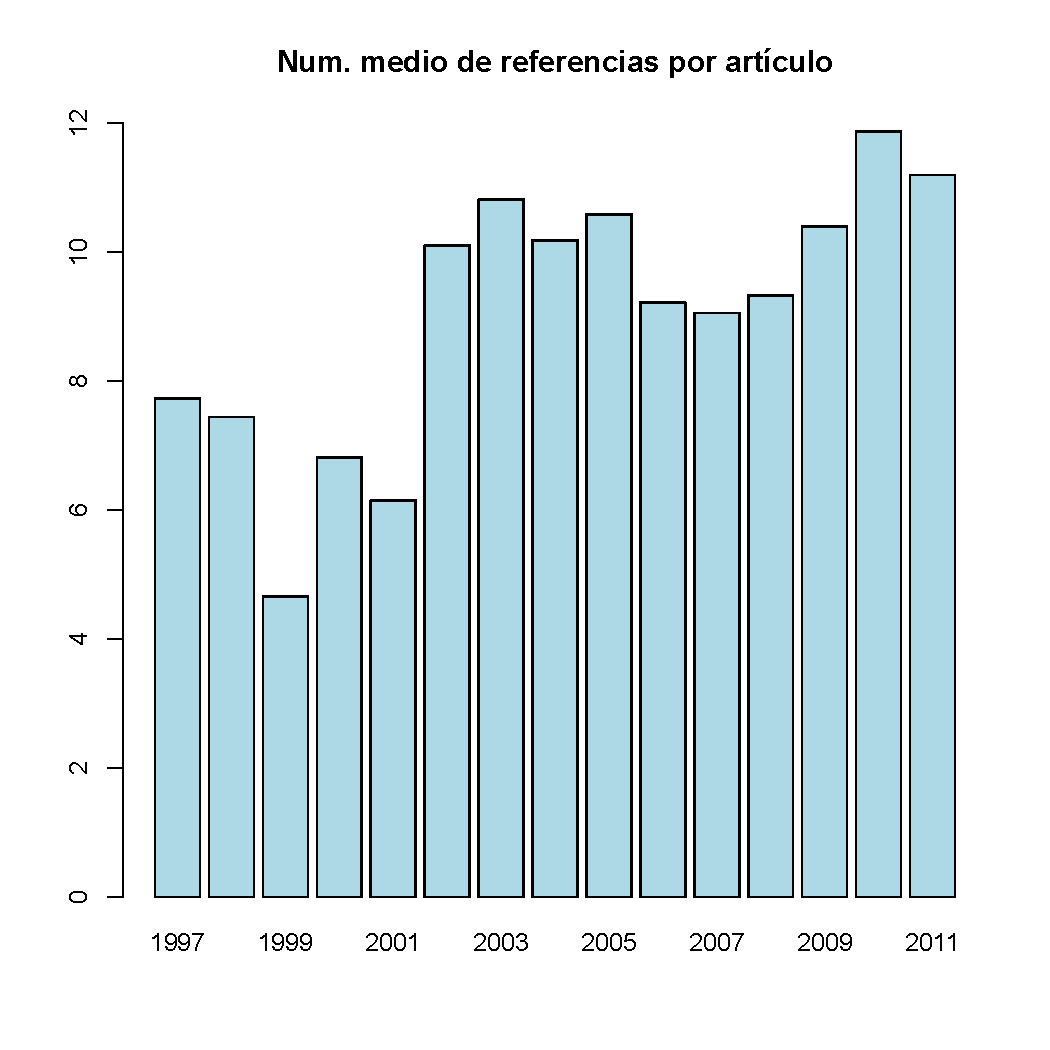
\includegraphics[width=\linewidth]{mediaref}}
%\caption{\label{fig:medias} Número medio de referencias por artículo en las 15 ediciones de las Jenui} 
%\label{fig:} 
%\end{figure}
%%%%%%%%%%%%%%%%%%%%%%%%%%%%%%%%%%%%%%%%%%%%%%%%%%%%%%%%%%%%%%

%%%%%%%%%%%%%%%%%%%% Fig. %%%%%%%%%%%%%%%%%%%%%%%%%%%%%%%%%%%
%\begin{figure*}
%	\begin{center}
%	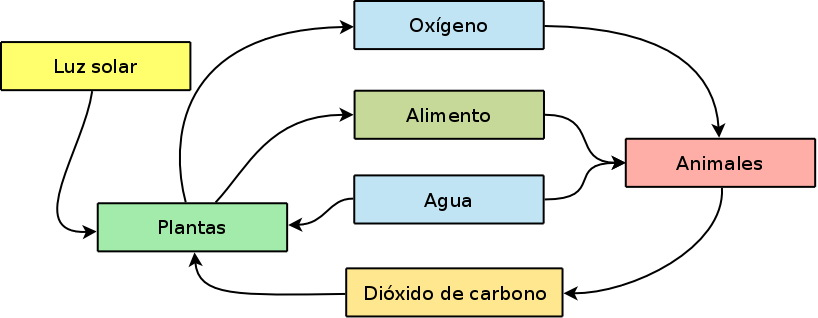
\includegraphics[width = 0.8\linewidth]{diagrLargo.jpg}
%	\end{center}
%	\caption{Diagrama en ancho de dos columnas.}
%\end{figure*}
%%%%%%%%%%%%%%%%%%%%%%%%%%%%%%%%%%%%%%%%%%%%%%%%%%%%%%%%%%%%%%

\end{document}
